%! Licence = CC BY-NC-SA 4.0

%! Author = mariuszindel
%! Date = 30. Jan 2022
%! Project = Cheat-Sheet-Web-Engineering-3


\section{SPA}

%-------------------------------------------------

%Lernziele:
%Unterschiede zwischen SPA und einer traditionellen Web Applikation
%die Konzepte MVC+S und Routing in einer SPA
%die wichtigsten Konzepte des Bundlings mit WebPack
%die Konzepte von Dependency Injection

%-------------------------------------------------

\subsection{Vor- und Nachteile}
\begin{itemize}[label={\textcolor{darkGreen}{+}}]
    \item Platform \& Device unabhängig
    \item Pay as you go (Software as a Service)
    \item Überall und immer auf allen Geräten verfügbar (keine Installation nötig)
    \item Keine Updates auf Client Seite
    \item Kein Page Reload (nur Daten aktualisieren)
\end{itemize}
\begin{itemize}[label={\textcolor{red}{--}}]
    \item Datenhoheit beim Anbieter
    \item Limitierte HW Zugriffe, weniger effizient
    \item SEO - Search engines must execute JavaScript
    \item Aufwendiger in der SW entwicklung
\end{itemize}

\subsection{Architektur}
\begin{center}
    \vspace{-4pt}
    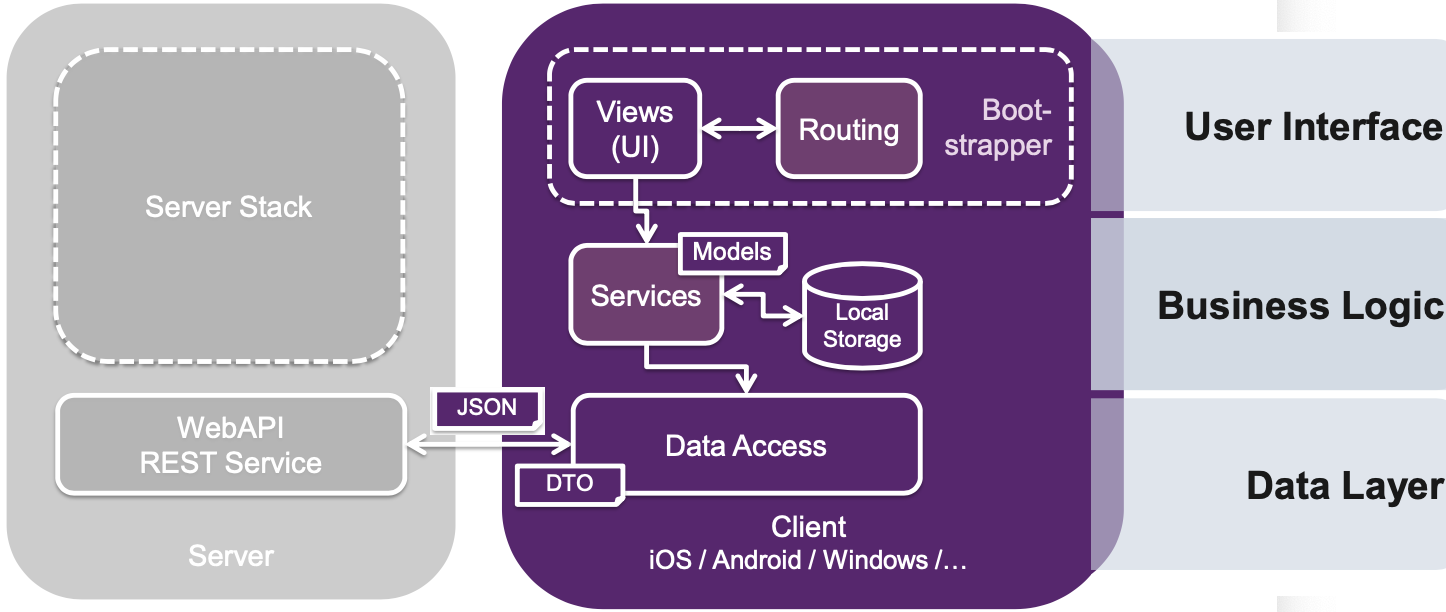
\includegraphics[width=1.02\linewidth]{./img/01-spa/architecture_layers}
    \vspace{-16pt}
\end{center}

%\subsubsection{Routing}

\subsection{Bundlings}

\subsubsection{Übersicht}
\begin{itemize}
    \item neuste Technologien Pre- und Post-Processors verwenden, ohne Browser Kompatibilität zu brechen
    \item Client-Side Code wird komplexer $\rightarrow$ Bundlers optimieren (TreeShaking, minifizieren)
    \item SPA ohne Bundlers $\rightarrow$ Build-Prozess muss von Hand geschrieben werden $\rightarrow$ schlecht wartbar
\end{itemize}

\subsubsection{Komponenten}
\begin{itemize}
    \item \textbf{Entry}
    Einstiegspunkt für webpack, folgt den Abhängigkeiten um zu bündeln
    \item \textbf{Output}
    Wo es Ihre Anwendung bündeln soll
    \item \textbf{Loaders}
    Loader (Modul/Regel-API) wandeln Dateien in Module um
    \item \textbf{Plugins}
    Aktionen und benutzerdefinierte Funktionen (Optimierung von Paketen, Verwaltung von Assets, Umgebungsvariablen)
    \item \textbf{Mode}
    Aktivierung von integrierten Optimierungsmechanismen.
\end{itemize}